\documentclass{standalone}
\usepackage{tikz}
\usepackage{tikzpeople}

\begin{document}
			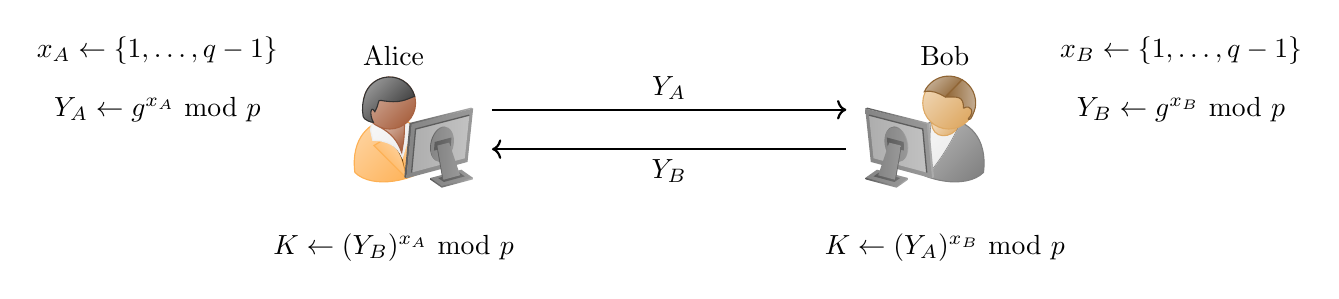
\begin{tikzpicture}
				
				\node[alice, monitor, label=Alice, minimum size=1cm] (Alice) at (0,0) {};
				\node[bob, mirrored, monitor, label=Bob, minimum size=1cm] (Bob) at (7,0) {};
				
				\draw[->, thick] (1.25,0.25)  -- (5.75,0.25) node[midway, above] {$Y_A$};
				\draw[<-, thick] (1.25,-0.25)  -- (5.75,-0.25) node[midway, below] {${Y_B}$};
				
				\node[] (AGen) at (-3,1) {${x_A} \gets \{1,\ldots,q-1\}$};
				\node[] (AEncap) at (-3,0.25) {${Y_A} \gets g^{{x_A}}$ mod $p$};
				\node[] (ADecap) at (0,-1.5) {${K} \gets ({Y_B})^{{x_A}}$ mod $p$};
				\node[] (BGen) at (10,1) {${x_B} \gets \{1,\ldots,q-1\}$};
				\node[] (BEncap) at (10,0.25) {${Y_B} \gets g^{{x_B}}$ mod $p$};
				\node[] (BDecap) at (7,-1.5) {${K} \gets ({Y_A})^{{x_B}}$ mod $p$};
				
			\end{tikzpicture}

\end{document}
